\comment{TODO}

\begin{figure}[!ht]
    \centering
    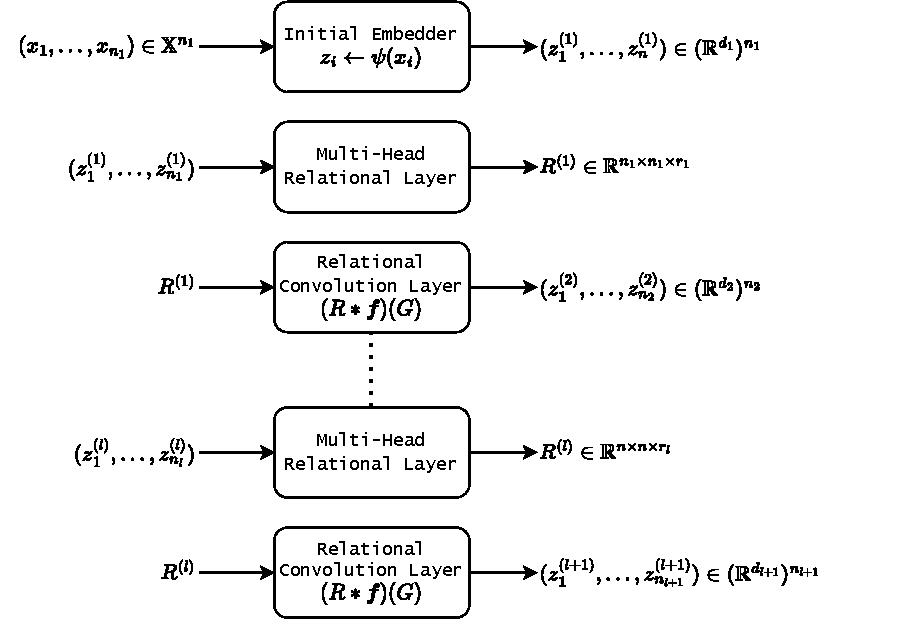
\includegraphics[width=0.75\textwidth]{figs/relational_framework.pdf}
    \caption{A depiction of our proposed framework for hierarchical relational machine learning. At each layer, the multi-head relation module takes a sequence of objects as input and produces a relation tensor representing the relations between each pair of objects. The relational convolution layer then transforms the relation tensor into a sequence of objects each describing the relations within some group of objects at the previous layer. The next layer receives this sequence of objects as input and again models the relations within it. Thus, each layer computes relational features of a higher-order (i.e., relations on relations). \textit{Legend}: $d_l$ represents the dimension of the objects at layer $l$; $z_i^{(l)}$ is the $i$th object at the $l$th layer; $R^{(k)}$ is the relation tensor at layer $l$; $r_l$ is the dimension of the relations at layer $l$; $n_l$ is the number of objects at layer $l$.}\label{fig:relational_framework}
\end{figure}
